\lhead[\thepage]{CHAPTER \thechapter. IMPLEMENTATION AND DEPLOYMENT}
\chead[]{}
\rhead[A Complete Simulator for Volunteer Computing Environments\leftmark]{\thepage}
\renewcommand{\headrulewidth}{0.5pt}

\lfoot[]{}
\cfoot[]{}
\rfoot[]{}
\renewcommand{\footrulewidth}{0pt}

%% This is an example first chapter.  You should put chapter/appendix that you
%% write into a separate file, and add a line \include{yourfilename} to
%% main.tex, where `yourfilename.tex' is the name of the chapter/appendix file.
%% You can process specific files by typing their names in at the 
%% \files=
%% prompt when you run the file main.tex through LaTeX.
\chapter{Implementación y despliegue}
\label{ch:implementation_and_deployment}
\markboth{}{IMPLEMENTATION}

This chapter deals with the implementation and deployment of the software. Regarding the implementation of the system, the more complicated parts of the code are explained (Section \ref{sec:implementation}, \textit{\nameref{sec:implementation}}). On the other hand, we explain the steps required to deploy the final system (Section \ref{sec:deployment}, \textit{\nameref{sec:deployment}}).

\section{Implementación}
\label{sec:implementation}

As we explained in Chapter \ref{ch:analysis}, \textit{\nameref{ch:analysis}}, we have implemented the simulator using the C programming language and the tools provided by SimGrid. The SimGrid core is responsible for planning the different processes, but the developer is the one that must use synchronization mechanisms to avoid race conditions. He have used several mutexes and condition variables in order to solve the problem of reading-writing in shared structures. 

Furthermore, we have worked so that the project servers simulated in ComBoS have a realistic behavior. To do this, we have divided the functioning of each server (both \gls{scheduling} and data servers) into two main processes: requests and \gls{dispatcher} (see Figure \ref{fig:server_processes}).

The \textit{requests} process is in charge of receiving all client requests through the corresponding mailbox. It receives messages asynchronously; that is, the process does not wait to finish receiving a message from a client in order to start receiving the next one. Each time a request is received, it is inserted into a queue that is shared with the \textit{\gls{dispatcher}} process. The \gls{dispatcher} process is responsible for dealing with requests and answering to the volunteer clients if necessary. Response messages are sent asynchronously as well.

\clearpage

\begin{figure}[htbp]
 	\centering
 	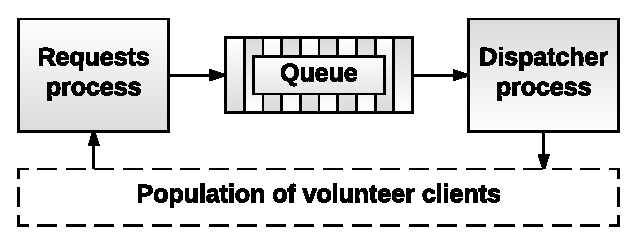
\includegraphics[width=12.5cm]{figures/server_processes}
 	\caption{Server main processes.}
	\label{fig:server_processes}
\end{figure}

\vspace{1cm}

On the other hand, each client is implemented with at least three different processes: the client main process (Pseudocode \ref{alg:client_main_thread}), which updates the client parameters every \gls{scheduling} interval; the work fetch process (Pseudocode \ref{alg:work_fetch_thread}), which selects the project to ask for work; and the execution processes, one per attached project, that execute the tasks. We have not included the pseudocode of the execution process because it only dequeues tasks and executes them. Our simulator is complemented with the most important features of the real scheduler (deadline \gls{scheduling}, long term debt, fair sharing and exponential back-off) as explained in Section \ref{sec:local_scheduling_policies}, \textit{\nameref{sec:local_scheduling_policies}} (Chapter \ref{ch:design}, \textit{\nameref{ch:design}}).

\vspace{1cm}

\begin{algorithm}[h]
	\caption{Client main process}
	\label{alg:client_main_thread}
  	\scriptsize
  	\setstretch{1.35}
	\begin{algorithmic}[1]
		\Function{client\_main}{ }
		\While {time < max\_time}
		\State increase $wall\_cpu\_time$ to the running project
		\State \Call{update\_debt}{}
		\State \Call{update\_deadline\_missed}{}
		\State \Call{cpu\_scheduling}{}
		\State \Call{signal}{} Work fetch process
		\State \Call{wait}{} $scheduling\_interval$
		\EndWhile	
		\State Return
		\EndFunction
	\end{algorithmic}
\end{algorithm}

\clearpage

\begin{algorithm}[h]
	\caption{Work fetch process}
	\label{alg:work_fetch_thread}
  	\scriptsize
  	\setstretch{1.35}
	\begin{algorithmic}[1]
		\Function{work\_fetch}{ }
		\State $project = null$
		\While {time < max\_time}
		\For {each project $p$ in $projects$}
		\If {$p$ meets the requirements}
		\State $project = p$
		\EndIf
		\EndFor
		\If {$project$ and not $deadlines\_missed$}
		\State \Call{ask\_for\_work}{$project$}
		\EndIf		
		\State \Call{wait}{} $work\_fetch\_period$
		\EndWhile	
		\State \Call{signal}{} Client main process
		\State Return
		\EndFunction
	\end{algorithmic}
\end{algorithm}


\section{Deployment}
\label{sec:deployment}

This section presents the deployment of the system. The technical specifications recommended for the final user to obtain the best experience from the application are:

\begin{itemize}

\item \textbf{Operating System}: Ubuntu 14.04.4 LTS (Linux distribution) or higher.

\item \textbf{Processor}: Intel(R) Core(TM) i7 CPU 920 @2.67GHz or higher.

\item \textbf{\gls{ram}}: 8 GB or higher.

\item \textbf{Storage}: 1 GB of free space in the Hard Disk Drive.

\item \textbf{Network}: Internet connection is not required.

\item \textbf{Software}: The following software must be installed in order to run the application:

	\begin{itemize}

	\item[1.] GCC (GNU Compiler) 5.1 or higher.
	
	\item[2.] SimGrid toolkit 3.10 or higher.
	
	\end{itemize}

\end{itemize}


To make life easier for the end user, we have organized the application files in the simplest way possible. Figure \ref{fig:folder_structure} shows the initial structure of the application files.

\begin{figure}[htbp]
 	\centering
 	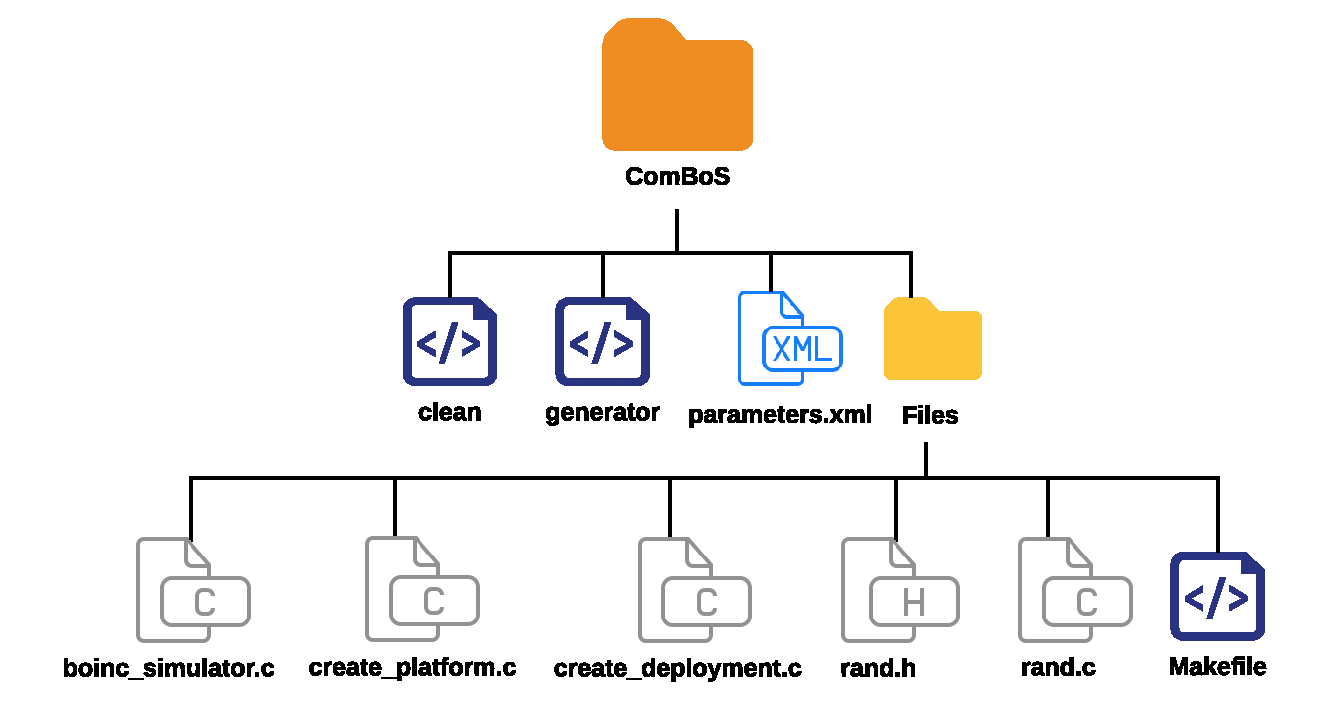
\includegraphics[width=15.5cm]{figures/folder_structure}
 	\caption{Initial folder structure.}
	\label{fig:folder_structure}
\end{figure}

The files located inside the \gls{comsimboinc} main folder are detailed below:

\begin{itemize}

\item \textbf{clean:} it is a script that removes the files created by the generator script.

\item \textbf{generator:} it is a script that generates all the files needed for the simulation based on the parameters specified in the parameters.xml file. The files created by this script are:

\begin{itemize}

\item \textbf{execute:} it is a script that executes the simulation (runs the file boinc\_simulator).

\item \textbf{Files/create\_platform:} it is the executable file that results from compiling the create\_platform.c file.

\item \textbf{Files/create\_deployment:} it is the executable file that results from compiling the create\_deployment.c file.

\item \textbf{Files/platform.xml:} platform file created by create\_platform. 

\item \textbf{Files/deployment.xml:} deployment file created by create\_deployment. 

\item \textbf{Files/boinc\_simulator:} it is the executable file that results from compiling the boinc\_ simulator.c and rand.c files.

\end{itemize}

\item \textbf{parameters.xml:} to create a simulation, \gls{comsimboinc} requires the specification of all the parameters needed in an \gls{xml} file, such as the simulation time in hours. All other parameters required by the \gls{xml} file are detailed in Tables \ref{tab:project_parameters} and  \ref{tab:vngroup_parameters} (presented in Chapter \ref{ch:design}, \textit{\nameref{ch:design}})

\item \textbf{Files:} folder that includes:

\begin{itemize}
\item \textbf{boinc\_simulator.c:} simulator main source code.
\item \textbf{create\_platform.c:} source code that contains the generation of the platform file.
\item \textbf{create\_deployment.c:} source code that contains the generation of the deployment file.
\item \textbf{rand.h:} header file for random functions.
\item \textbf{rand.c:} source code that contains the random functions.
\item \textbf{Makefile:} script that compiles and links the code files.
\end{itemize}

\end{itemize}


The Appendix \ref{ch:user_manual} presents a complete user manual of the simulator. It includes a tutorial for the installation of the SimGrid toolkit, and a number of practical and educational examples to learn how to perform simulations. In a basic way, in order to deploy the application, the user only needs to follow the following steps:

\begin{itemize}

\item Download the main folder of the \gls{comsimboinc} application (of which the structure is presented in Figure \ref{fig:folder_structure}).

\item Indicate the simulation parameters in the parameters \gls{xml} file. This file must include all the parameters specified in Tables \ref{tab:project_parameters} and \ref{tab:vngroup_parameters} (presented in Chapter \ref{ch:design}, \textit{\nameref{ch:design}}).

\item Generate all the simulation files required, by just running the generator script.

\item Run the execution script.

\end{itemize}

\afterpage{\blankpage} % blank page